%%%%%%%%%%%%%%%%%%%%%%%%%%%%%%%%%%%%%%%%%
% Beamer Presentation
% LaTeX Template
% Version 1.0 (10/11/12)
%
% This template has been downloaded from:
% http://www.LaTeXTemplates.com
%
% License:
% CC BY-NC-SA 3.0 (http://creativecommons.org/licenses/by-nc-sa/3.0/)
%
%%%%%%%%%%%%%%%%%%%%%%%%%%%%%%%%%%%%%%%%%

%----------------------------------------------------------------------------------------
%	PACKAGES AND THEMES
%----------------------------------------------------------------------------------------

\documentclass[9pt]{beamer}

\mode<presentation> {

\usetheme{Berlin}

%\setbeamertemplate{footline} % To remove the footer line in all slides uncomment this line
\setbeamertemplate{footline}[page number] % To replace the footer line in all slides with a simple slide count uncomment this line

%\setbeamertemplate{navigation symbols}{} % To remove the navigation symbols from the bottom of all slides uncomment this line
}

\usepackage{graphicx} % Allows including images
\usepackage{tikz} % For precise overlay placement
\usepackage{booktabs} % Allows the use of \toprule, \midrule and \bottomrule in tables
\usepackage{verbatim} % Allows verbatim environments for code
\usepackage{textcomp} % Allows correct display of text in \texttt{}

\usepackage{listings}
\usepackage{xcolor}

\definecolor{darkgreen}{rgb}{0.0, 0.5, 0.0}  % Dark Green
\definecolor{darkpurple}{rgb}{0.5, 0.0, 0.5} % Dark Purple
\definecolor{verylightblue}{rgb}{0.95, 0.98, 1}

\lstdefinestyle{mystyle}{
    language=C++,
    linewidth=1.02\textwidth,
    basicstyle=\ttfamily\footnotesize,
    keywordstyle=[1]\color{darkgreen}\bfseries, % C++ keywords
    keywordstyle=[2]\color{blue}, % alpaka related keywords
    identifierstyle=\color{black},
    commentstyle=\fontfamily{dvs}\selectfont\color{gray}, % Using Inconsolata for comments
    stringstyle=\color{red},
    numberstyle=\tiny\color{gray},
    backgroundcolor=\color{verylightblue},
    numbers=left,
    numbersep=10pt,
    tabsize=2,
    breaklines=true,
    showstringspaces=false,
    escapeinside={(*@}{@*)},
    alsoletter={:}, % treat ':' as part of a keyword
    morekeywords={[1]auto, using, namespace, nullptr, static_cast, int, float, double, size_t, for, if, else, while, return}, % C++ keywords
    morekeywords={[2]alpaka, alpaka::PlatformCpu, alpaka::Vec, alpaka::Buf, alpaka::DevCpu, alpaka::Dev, alpaka::Platform, alpaka::KernelCfg, alpaka::WorkDivMembers, alpaka::AccGpuCudaRt, alpaka::AccGpuHipRt, alpaka::AccCpuThreads, alpaka::AccCpuOmp2Threads, alpaka::AccCpuOmp2Blocks, alpaka::AccCpuTbbBlocks, alpaka::AccCpuSerial, alpaka::AccGpuCudaRt, ALPAKA_FN_ACC} % alpaka keywords
}

\lstset{style=mystyle}

% Add footer with section and subsection
\setbeamertemplate{footline}{%
  \leavevmode%
  \hbox{%
  \begin{beamercolorbox}[wd=.5\paperwidth,ht=2.25ex,dp=1ex,left]{title in head/foot}%
    \usebeamerfont{title in head/foot}\hspace*{2ex}\insertsection\ :: \insertsubsection
  \end{beamercolorbox}%
  \begin{beamercolorbox}[wd=.5\paperwidth,ht=2.25ex,dp=1ex,right]{date in head/foot}%
    \usebeamerfont{date in head/foot}\insertframenumber{} / \inserttotalframenumber\hspace*{2ex}
  \end{beamercolorbox}}%
  \vskip0pt%
}

%----------------------------------------------------------------------------------------
%	TITLE PAGE
%----------------------------------------------------------------------------------------

% Redefine the headline to remove the blue line but keep space for logos
\setbeamertemplate{headline}{
    % Here, we can leave it empty or customize further, like adding section titles or navigation
    \vspace{1cm} % Keep some space for the logos to appear properly
}

% Overlay two logos using TikZ
\setbeamertemplate{background}{%
    \begin{tikzpicture}[remember picture,overlay]
        % Only show the Alpaka logo if it's NOT the title page or the last slide

            % Top right logo (logoAlpaka) with vertical adjustment
            \node[anchor=north east] at ([yshift=+0.1cm,xshift=+0.1cm]current page.north east) {\includegraphics[width=2.3cm]{logoCasus.png}};


        % Bottom left logo (logoCasus) appears on all slides
        \node[anchor=north west] at ([yshift=0cm] current page.north west) {\includegraphics[width=1.85cm]{logoAlpaka.png}};
    \end{tikzpicture}
}

\title{Alpaka Hackathon Section-II: Heat Equation Solution} % The short title appears at the bottom of every slide, the full title is only on the title page

\author{PLASMA-PEPSC Workshop on Alpaka and OPENPMD} % Your name
\institute[HZDR] % Your institution as it will appear on the bottom of every slide, may be shorthand to save space
{
\\ % Your institution for the title page
\medskip
\textit{} % Your email address
}
\date{\today} % Date, can be changed to a custom date

\begin{document}

\begin{frame}
\titlepage % Print the title page as the first slide
\end{frame}
\section{Section-II Introduction}
\subsection{Schedule}
\begin{frame}[t]{Workshop Schedule} % [t] aligns the top of the columns

\begin{columns}[T] % The [T] option aligns the tops of the columns
\vspace{-1.3cm}
\hspace*{-0.6cm} % Adjust the -1cm to move more or less to the left
% First Column
\begin{column}{0.44\textwidth}
\textbf{\small Section - I}

\begin{enumerate}
\color{gray}
    \item \small Introduction: What is alpaka, where it is used?
    \item \small \textbf{Hands on 1}: Installing alpaka and running an example (LUMI)
    \item \small Parallel programming concepts and portable parallelization by alpaka
    \begin{itemize}
    \color{gray}
        \item \scriptsize Grid Structure and WorkDivision
        \item \scriptsize Data Parallelism
        \item \scriptsize Indexing
    \end{itemize}
    \item \small \textbf{Hands on 2}: HelloIndex kernel which prints indexes
\end{enumerate}
\end{column}

% Second Column
\begin{column}{0.56\textwidth}
\textbf{\small Section - II}
\begin{enumerate}
    \item \small Memory management for 1D and 2D data
    \item \small Filling buffers in parallel
    \item \small \textbf{Hands on 3}: Kernel to fill initial conditions of heat equation
    \item \small Heat Equation
    \item \small Preparing stencil kernel
    \item \small \textbf{Hands on 4}: Heat Equation stencil kernel
    \item \small Programming features and data-structures of alpaka
    \item \small Usability and Optimization
    \begin{itemize}
        \item \scriptsize Using alpaka mdspan for easier indexing
              \textbf{Hands on 5}
        \item \scriptsize Domain Decomposition
              \textbf{Hands on 6} (Day2)
        \item \scriptsize Using async queues for performance increase
              \textbf{Hands on 7} (Day2)
        \item \scriptsize Using shared memory for performance increase
              \textbf{Hands on 8} (Day2)
    \end{itemize}
\end{enumerate}
\end{column}

\end{columns}
\end{frame}


%\subsection{Overview}
%\begin{frame}
%\frametitle{Overview of Section-II} % Table of contents slide
%\tableofcontents % Automatically prints the table of contents based on \section{} and \subsection{} commands
%\end{frame}

\section{Filling a buffer in parallel}
\subsection{Steps}
\begin{frame}
\frametitle{Steps of Filling a Buffer in Parallel}
\begin{columns}

    % First column
    \begin{column}{0.55\textwidth} % 50% of the width
    \begin{enumerate}
     \item Select the accelerator
     \item Create host-device, acc-device and the queue
     \item Allocate host and device memory using Buf and Vec data structures
     \item Decide how to parallelize: Set the work-division
     \item Create the kernel instance for filling the buffer
     \item Execute the kernel
     \item Copy the result from Acc (e.g GPU) back to the host buffer.
    \end{enumerate}
    \end{column}

    % Second column
    \begin{column}{0.45\textwidth} % 50% of the width
        \centering
        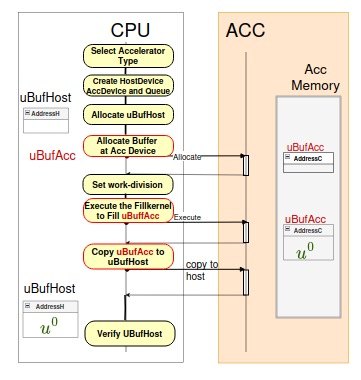
\includegraphics[width=\linewidth]{Screenshot from 2024-10-20 23-39-02.png} % Replace with your image
        %\caption{Filling A Buffer in Parallel}
    \end{column}

\end{columns}


    \end{frame}

%----------------------------------------------------------------------------------------
%	PRESENTATION SLIDES
%----------------------------------------------------------------------------------------

%------------------------------------------------
%------------------------------------------------
\subsection{Data Allocation and Pass}


 \begin{frame}[fragile]
 \vspace{-0.2cm}
\frametitle{Allocate memory at Host and at Device}
\textbf{Define number of dim and index type}
\begin{lstlisting}
using Dim = alpaka::DimInt<2u>; // Number of dim: 2 as a type
using Idx = std::size_t; // Index type of the threads and buffers
 \end{lstlisting}

\textbf{Define extents for buffers}
\begin{lstlisting}
   // alpaka::Vec is a static array similar to std::array.
   // Dim is a compile-time constant, which is 2.
    constexpr alpaka::Vec<Dim, Idx> numNodes{64, 64};
    constexpr alpaka::Vec<Dim, Idx> haloSize{2, 2};
    constexpr alpaka::Vec<Dim, Idx> extent = numNodes + haloSize;
\end{lstlisting}

\textbf{Allocate memories at host and accelerator}
\begin{lstlisting}
    // Allocate memory for host-buffer. Creates alpaka::Buf.
    auto uBufHost = alpaka::allocBuf<double, Idx>(devHost, extent);

    // Allocate memory for accelerator buffer
    auto uBufAcc = alpaka::allocBuf<double, Idx>(devAcc, extent);
\end{lstlisting}
\textbf{Pass acc pointer uBufAcc to kernel and execute kernel}
\begin{lstlisting}
alpaka::exec<Acc>(queue, workDiv, initBufKernel, uBufAcc.data(), ...);
\end{lstlisting}
\end{frame}

\begin{frame}[fragile]
\frametitle{Aim: Finding the adress of a data and fill it with a specific value}
\hspace{-0.4\baselineskip}
\textbf{Lets assume that the 2D data is a 15 rows x 7 columns matrix}
\newline

\begin{figure}
\hspace{-1.2\baselineskip}
   \centering
   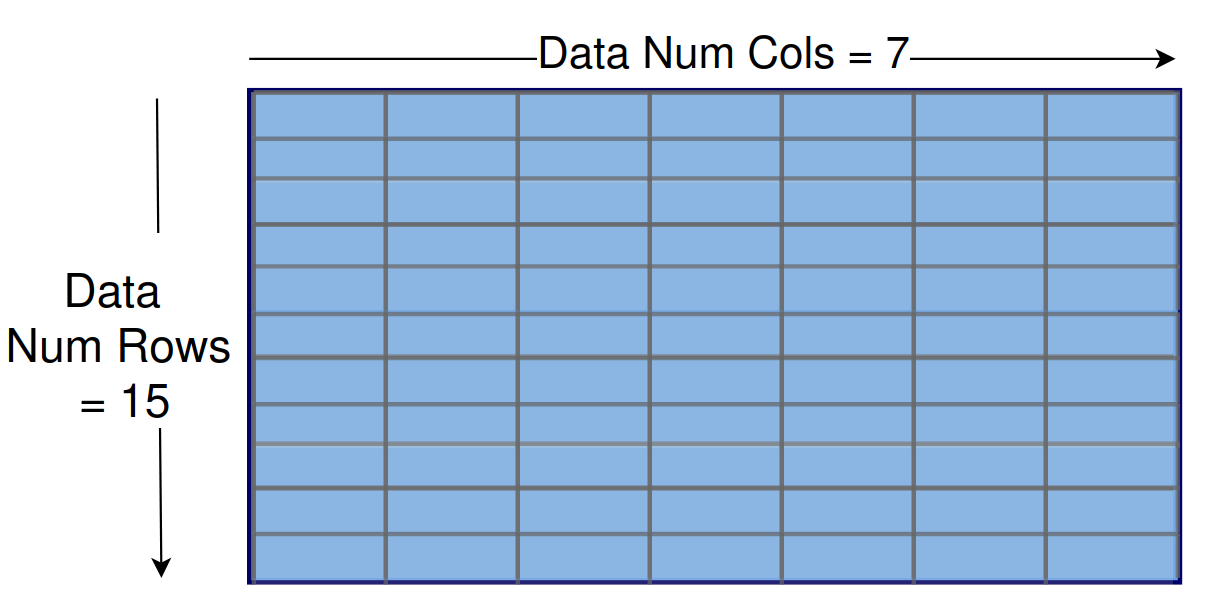
\includegraphics[width=0.45\linewidth]{Screenshot from 2024-10-21 01-01-17.png}
   \label{fig:enter-label}
\end{figure}
\hspace{0.1\baselineskip}
\small
\textbf{Assume that data-size is 3}
\begin{figure}
\hspace{-1.2\baselineskip}
   \centering
   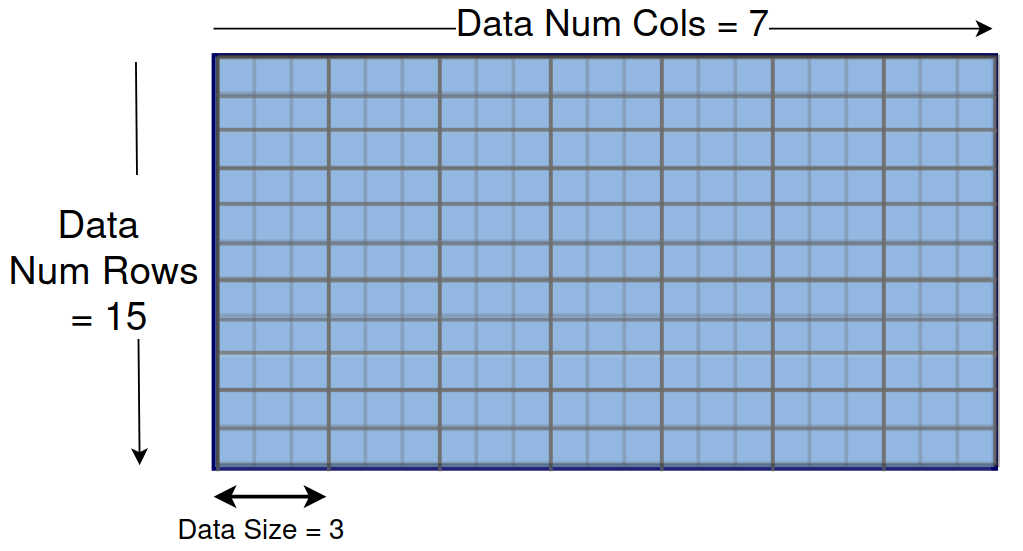
\includegraphics[width=0.45\linewidth]{Screenshot from 2024-10-21 00-56-34.png}
   \label{fig:enter-label}
\end{figure}

\end{frame}

\begin{frame}[fragile]
\frametitle{Structure of allocated data at the memory}
\hspace{-0.4\baselineskip}
\textbf{To fill the acc data buffer at the kernel the allocated memory structure should be known.}
\begin{figure}
\hspace{-1.2\baselineskip}
   \centering
   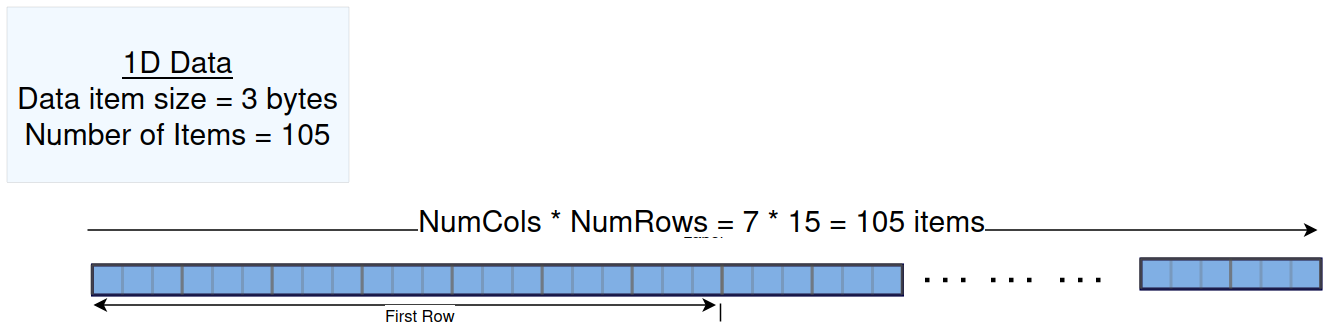
\includegraphics[width=0.75\linewidth]{Screenshot from 2024-10-21 01-36-15.png}
   \label{fig:enter-label}
\end{figure}
\hspace{0.1\baselineskip}
\begin{figure}
\hspace{-1.1\baselineskip}
   \centering
   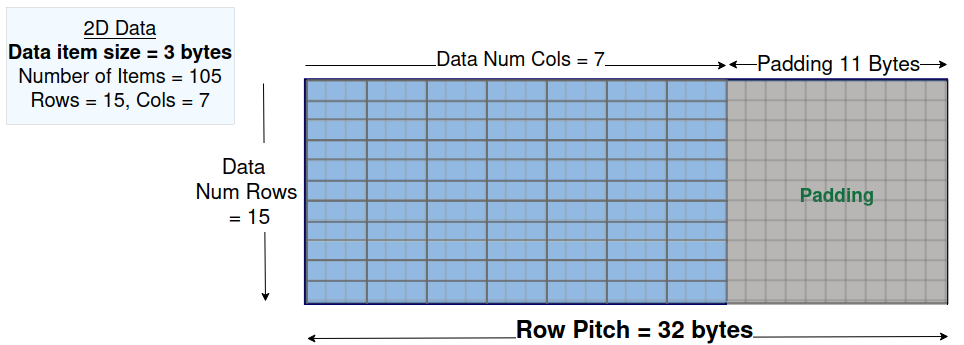
\includegraphics[width=0.75\linewidth]{Screenshot from 2024-10-01 17-30-50.png}
   \label{fig:enter-label}
\end{figure}
\end{frame}



\begin{frame}[fragile]
\frametitle{How to access data given the pointer and the pitch?}
\begin{figure}
    \centering
    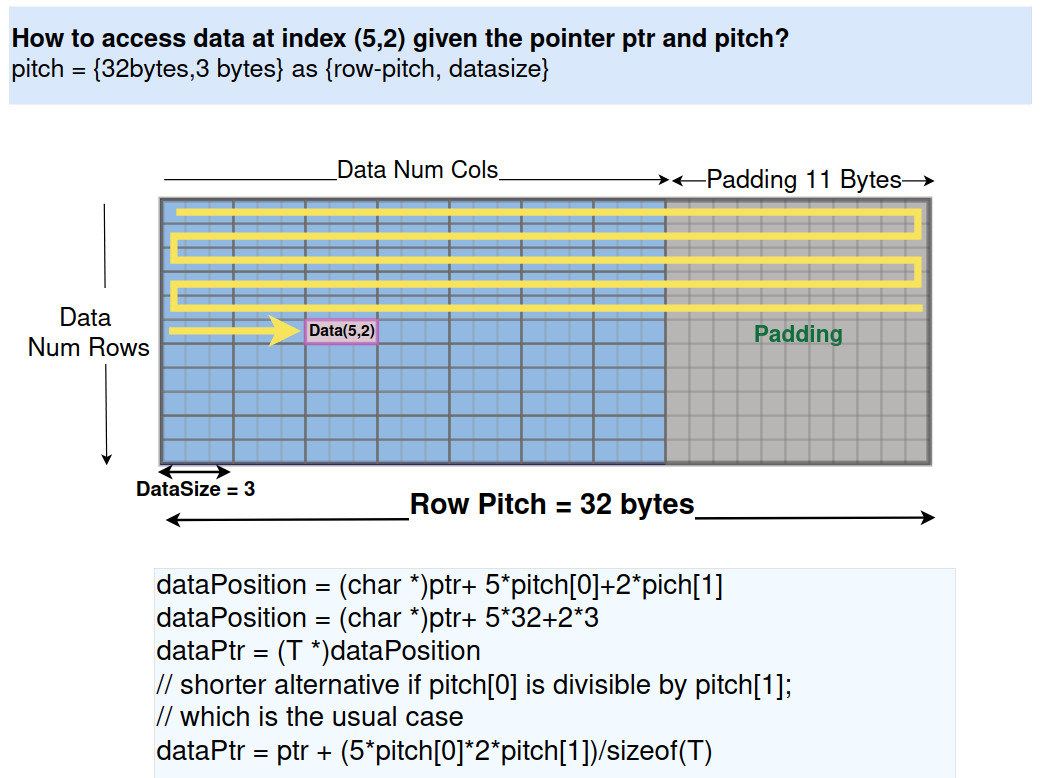
\includegraphics[width=0.80\linewidth]{Screenshot from 2024-10-02 15-47-27.png}
\end{figure}

\end{frame}


\begin{comment} %%%%%%%%%%%%%%%%%%%%%%
 \begin{frame}[fragile]
\frametitle{Copy the data to the device, use alpaka::Queue}

\begin{lstlisting}
    using Acc = alpaka::AccCpuSerial<Dim, Idx>;
    auto const platformAcc = alpaka::Platform<Acc>{};
    auto const devAcc = alpaka::getDevByIdx(platformAcc, 0);
    // A queue is needed for all acc related operations
    alpaka::Queue<Acc, alpaka::Blocking> queue(devAcc);

    // Define the 2D extents (dimensions)
    Vec const extentA(static_cast<Idx>(M), static_cast<Idx>(K));

    // Allocate host memory, the memory size is determined by extent
    auto bufHostA = alpaka::allocBuf<DataType, Idx>(devHost, extentA);

    // Allocate device memory
    auto bufDevA = alpaka::allocBuf<DataType, Idx>(devAcc, extentA);

    // Copy data to device, use host buffer and device buffer
    // Queue must be an accelerator queue
    alpaka::memcpy(queue, bufDevA, bufHostA);

\end{lstlisting}
\end{frame}
\end{comment} %%%%%%%%%%%%%%%%%%%%%%%%%%%%%%%

\begin{frame}[fragile]
\small
\frametitle{Passing multi dimensional buffer to the kernel}
 \begin{itemize}
 \item \textbf{Pass 3 variables for a buffer: pointer,  "row-pitch", and datasize}

If a pointer of a 2D buffer is passed to the kernel as a pointer; 2 additional values \textbf{pitch} and item \textbf{data-size} should also be passed.

        \lstset{basicstyle=\ttfamily\scriptsize}
        \begin{lstlisting}
    // Signature of function operator of the Kernel
    template<typename TAcc, typename TDim, typename TIdx>
    ALPAKA_FN_ACC auto operator()(
        TAcc const& acc,
        double* const bufData,
        // 2 variables row-pitch and data-type size
        alpaka::Vec<TDim, TIdx> const pitch,
        double dx,
        double dy) const -> void
        \end{lstlisting}

        \hspace{-0.2\baselineskip}


\item \textbf{Simple Alternative:} Pass an \textbf{alpaka mdspan} object
\lstset{basicstyle=\ttfamily\scriptsize}
\begin{lstlisting}
    template<typename TAcc, typename TDim, typename TIdx, typename TMdSpan>
    ALPAKA_FN_ACC auto operator()(
        TAcc const& acc,
        TMdSpan uAccMdSpan
        ...) const -> void
\end{lstlisting}
\end{itemize}
\end{frame}



\subsection{Hands on 3: InitilizeBuffer Kernel}
%----------------------------------------------

\begin{frame}
\frametitle{The Kernel to Initialize Heat Values}
\textbf{Calculate and set initial heat values, the $u^{0}$ matrix, by running a grid of threads.}
\hspace{2.0\baselineskip}
\begin{figure}
    \centering
    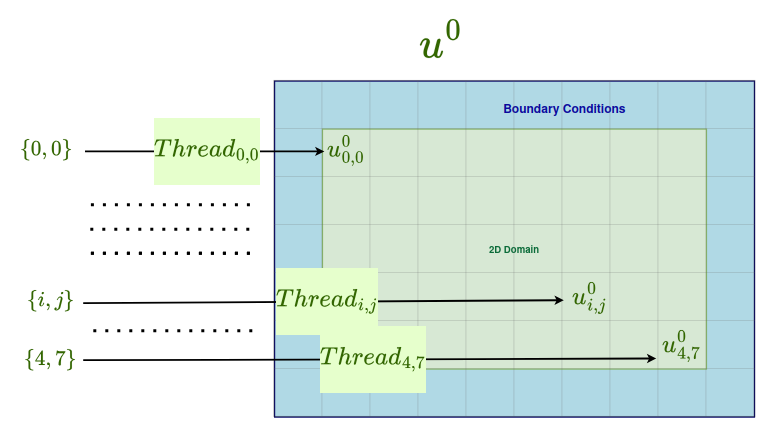
\includegraphics[width=0.8\linewidth]{Screenshot from 2024-09-19 18-45-43.png}
    \label{fig:enter-label}
\end{figure}
\end{frame}

\begin{frame}[fragile]
\frametitle{Hands on 3: The Kernel to Initialize Heat Values}
\small

\textbf{ The \textit{InitializeBufferKernel} fills the given buffer at the accelerator device (e.g GPU)}
    \lstset{basicstyle=\ttfamily\scriptsize}
    Prepare kernel to set initial heat values
    \begin{itemize}
    \item \textbf{Thread Index:} Find thread index in the kernel to be used as index to set 2D buffer.
    \item \textbf{Initial Condition at the point:} Find analytically the heat value at the point which has coordinates equal to the 2D thread index.
    \item \textbf{Memory Adress in Buffer:} Calculate the corresponding memory adress in buffer using thread index. Take into account the row-pitch and data-size
    \item \textbf{Set Value at the Adress:} Set the data at the memory position to the calculated initial condition.
    \end{itemize}
     \lstset{basicstyle=\ttfamily\tiny}
    \begin{lstlisting}
    template<typename TAcc, typename TDim, typename TIdx>
    ALPAKA_FN_ACC auto operator()(
        TAcc const& acc, double* const bufData,
        alpaka::Vec<TDim, TIdx> const pitch, double dx, double dy) const -> void {
    // Get 2D thread index using alpaka index function
    .....
    // Calculate analytical solution at point
    auto heatAtPointValue = analyticalSolution(acc, gridThreadIdx[1] * dx, gridThreadIdx[0] * dy, 0.0);
    // Calculate data position in buffer, from thread index and pitches
    auto ptr = getElementPtr(bufData, gridThreadIdx, pitch);
    // Set the value using the adress
    *ptr    = heatPointValue;
    } // function operator
    \end{lstlisting}

\end{frame}

%------------------------------------------------

%------------------------------------------------
% mention dont provide code or detailed info



\begin{frame}
\frametitle{Hands-On Session}
\begin{center}
      \Huge \textbf{Hands-on Session3: Filling an accelerator buffer paralelly}
  \end{center}
\end{frame}

%------------------------------------------------
\section{Introduction for Heat Equation} % Sections can be created to organize your presentation into discrete blocks
%------------------------------------------------
\subsection{Difference Equation}
\begin{frame}
\vspace{-0.1\baselineskip} % This moves the text up by approximately two lines

\frametitle{The Heat Equation}
\scriptsize
\begin{itemize}
    \item \textbf{The Heat Diffusion over time:}
    \fcolorbox{white}{verylightblue}{
    \parbox{0.50\textwidth}{
    \[
    \frac{\partial u(x, y, t)}{\partial t} = \alpha \left( \frac{\partial^2 u(x, y, t)}{\partial x^2} + \frac{\partial^2 u(x, y, t)}{\partial y^2} \right)
    \]
    } }
\newline % Adjust the vertical space as needed
\textbf{Time and Spatial Derivative Approximations:}
\newline
\begin{minipage}{0.45\textwidth}

     \[
\frac{\partial u(x, y, t)}{\partial t}\Bigg|_{t = t^n} \approx \frac{u_{i,j}^{n+1} - u_{i,j}^n}{\Delta t}
\]
\end{minipage}
\begin{minipage}{0.45\textwidth}

\[
\frac{\partial^2 u(x, y, t)}{\partial x^2}\Bigg|_{x = x_i, y = y_j} \approx \frac{u_{i+1,j}^n - 2u_{i,j}^n + u_{i-1,j}^n}{\Delta x^2}
\]
\end{minipage}
\item \textbf{Resulting difference equation:}
\[
u_{i,j}^{n+1} = u_{i,j}^n + \alpha \Delta t \left( \frac{u_{i+1,j}^n - 2u_{i,j}^n + u_{i-1,j}^n}{\Delta x^2} + \frac{u_{i,j+1}^n - 2u_{i,j}^n + u_{i,j-1}^n}{\Delta y^2} \right)
\]
\end{itemize}
\vspace{-0.5\baselineskip}
\begin{figure}
    \centering
    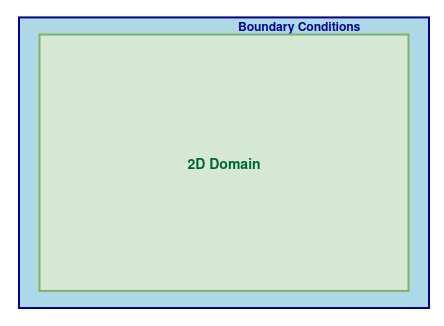
\includegraphics[width=0.50\linewidth,height=0.30\linewidth]{Screenshot from 2024-08-30 14-04-56.png}
\end{figure}
\end{frame}

\subsection{Stencil Matrix}
\begin{frame}
\vspace{-0.1\baselineskip} % This moves the text up by approximately two lines

\frametitle{The Heat Equation- Cont.}
\scriptsize
\begin{itemize}
\item \textbf{The difference equation:}
\[
u_{i,j}^{n+1} = u_{i,j}^n + \alpha \Delta t \left( \frac{u_{i+1,j}^n - 2u_{i,j}^n + u_{i-1,j}^n}{\Delta x^2} + \frac{u_{i,j+1}^n - 2u_{i,j}^n + u_{i,j-1}^n}{\Delta y^2} \right)
\]
\item \textbf{Substitute:}
\vspace{0.3\baselineskip}
 \( \alpha = 1 \), \( r_X = \frac{\Delta t}{\Delta x^2} \), \( r_Y = \frac{\Delta t}{\Delta y^2} \) . \textbf{Then \( u_{i,j}^{n+1} \) is:}

\[
u_{i,j}^{n+1} = u_{i,j}^n + r_X \left( u_{i+1,j}^n - 2u_{i,j}^n + u_{i-1,j}^n \right) + r_Y \left( u_{i,j+1}^n - 2u_{i,j}^n + u_{i,j-1}^n \right)
\]

By regrouping the terms related to \( u_{i,j}^n \), the equation can be rewritten as:
\fcolorbox{white}{verylightblue}{
\parbox{0.85\textwidth}{
\[
u_{i,j}^{n+1} = u_{i,j}^n \left( 1 - 2r_X - 2r_Y \right) + r_X \left( u_{i+1,j}^n + u_{i-1,j}^n \right) + r_Y \left( u_{i,j+1}^n + u_{i,j-1}^n \right)
\] }}
\end{itemize}
\vspace{-0.7\baselineskip}
\begin{columns}
\begin{column}{0.40\textwidth}
\[
S= \begin{pmatrix}
0   & r_{Y}   & 0 \\
r_{X}  & 1 - 2r_{X} - 2r_{Y}  & r_{X} \\
0   & r_{Y}   & 0
\end{pmatrix}
\]
\end{column}

\begin{column}{0.60\textwidth}
\begin{figure}
    \centering
    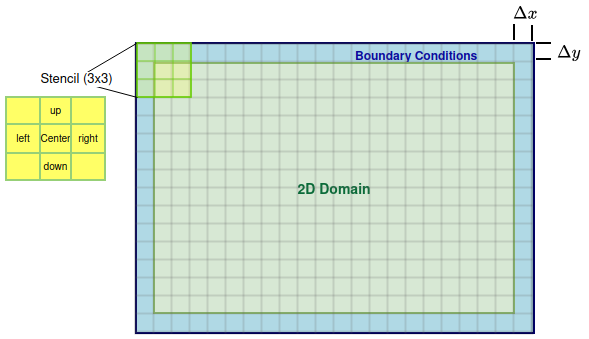
\includegraphics[width=0.90\linewidth, height=0.50\linewidth]{Screenshot from 2024-09-30 14-37-35.png}
\end{figure}
\end{column}
\end{columns}
\end{frame}

\section{Parallel Solution of Heat Eqn.}

%------------------------------------------------
\subsection{Domain and Stencil}
%------------------------------------------------
% All domain etc
\begin{frame}
\frametitle{Parallel Heat Equation Solution}
\vspace{-0.5\baselineskip}
\scriptsize
    \begin{itemize}
        \item \textbf{Data Parallelism:} Each point on the grid can be updated independently based on its neighbors, enabling parallel computation.
        \item \textbf{Independency:} Next values of heat at a point does not depend on previous heat values.
        \item \textbf{Stencil Operations:} Stencil is a core computational pattern in PDE solvers. Updates a grid point in time using its immediate neighbors (left, right, up, down) according to the difference equation.
    \end{itemize}
    %first image without blocks
    \vspace{-0.5\baselineskip}
    \begin{figure}
        \centering
        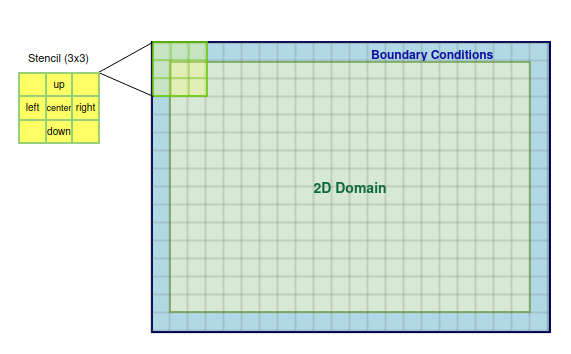
\includegraphics[width=0.6\linewidth]{Screenshot from 2024-08-30 14-18-30.png}
        \label{fig:enter-label}
    \end{figure}
    \begin{itemize}
        \item \textbf{Halo Region for BC:} A layer of grid cells added to the core-domain surrounding the problem domain for Boundary Conditions.
       \end{itemize}

\end{frame}


\begin{frame}
\frametitle{Halo Region}
\vspace{-0.5\baselineskip}
\scriptsize
    %first image without blocks
    \vspace{-0.5\baselineskip}
    \begin{figure}
        \centering
        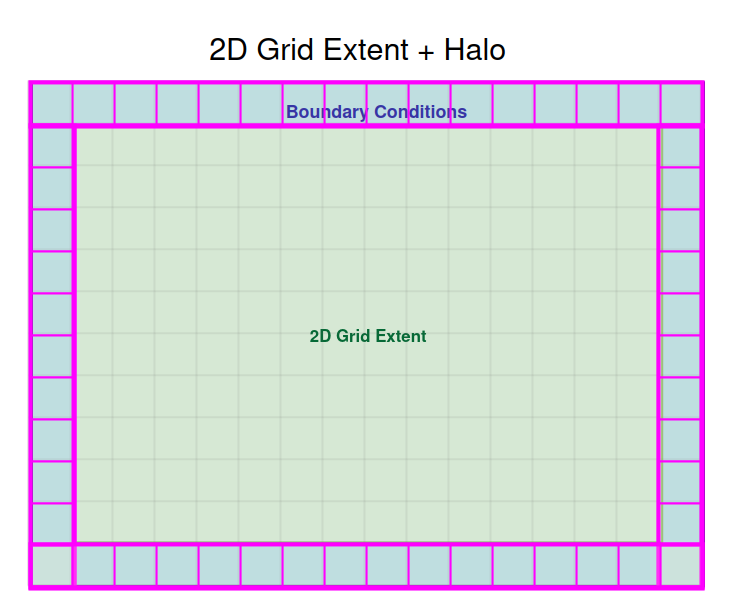
\includegraphics[width=0.6\linewidth]{Screenshot from 2024-10-22 01-51-12.png}
        \label{fig:enter-label}
    \end{figure}

\end{frame}


\begin{frame}
\frametitle{Calculation of $u_{i,j}^{n+1}$ from $u_{i,j}^{n}$}
\vspace{-0.1\baselineskip}
    \begin{itemize}
        \item Kernel execution by thread ${i,j}$  calculates $u_{i,j}^{n+1}$ using $u_{i,j}^{n}$
        \item Hence, Each heat point is separately calculated by a thread using \textbf{Frobenious Inner Product} (FIP) of \( S \) and matrix \( U_{i,j} \):
\[
 u_{i,j}^{n+1} = \langle S, U^{n}_{i,j} \rangle_F = \sum_{m=1}^{M} \sum_{k=1}^{K} s_{m,k} u_{m,k}
\]
        \item $S$ and $U^{n}_{0,0}$ is used  by a thread to calculate $u_{0,0}^{n+1}$ using FIP
    \end{itemize}
    \begin{figure}
        \centering
            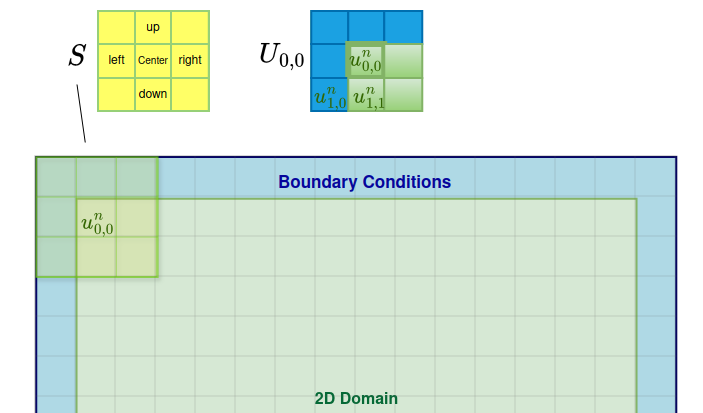
\includegraphics[width=0.75\linewidth, height=0.4\textheight]{Screenshot from 2024-09-22 00-16-53.png}
             %   \caption{First thread calculates $u_{0,0}^{n+1}$ using \textbf{Frobenious Inner Product} of 3x3 matrices}
        \label{fig:enter-label}
    \end{figure}
\end{frame}

\begin{frame}
\vspace{-0.9\baselineskip}
    \begin{itemize}
        \item Another thread calculates $u_{0,1}^{n+1}$  using $S$ and $U^{n}_{0,1}$
    \end{itemize}
    \begin{figure}
        \centering
        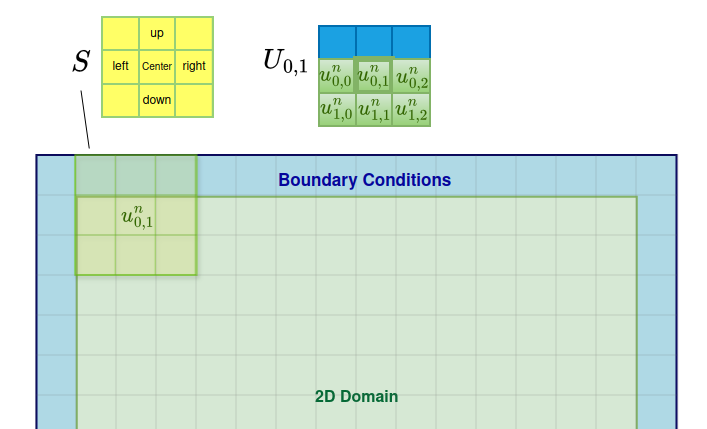
\includegraphics[width=0.8\linewidth,height=0.45\linewidth]{Screenshot from 2024-09-21 23-44-50.png}
        \caption{Another thread calculates $u_{0,1}^{n+1}$ }
        \label{fig:enter-label}
    \end{figure}
\end{frame}

\subsection{Indexing of Stencil Kernel}
\begin{frame}
\frametitle{A grid of threads is used to find next 2D heat values}
\begin{figure}
    \centering
    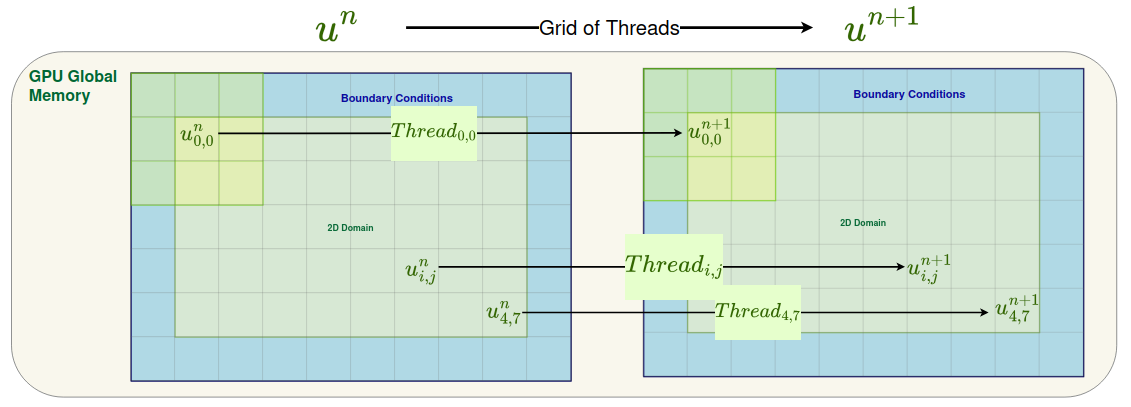
\includegraphics[width=0.86\linewidth]{Screenshot from 2024-10-02 16-04-45.png}
\end{figure}

\begin{itemize}
    \item Stencil kernel will update only core nodes not the border
    \item The workdiv for stencil-kernel can be calculated by setting grid-thread extent to nodes domain
    \item The workdiv for the borders-kernel would need larger extents, but will only work on borders of this extended domain.    %\item Some threads other than the ones updating the border will do nothing when running Boundary kernel
\end{itemize}


\end{frame}

% FULL SOLUTION INCLUDING SHARED
%\subsection{All Solution Steps}
%\begin{frame}
%\frametitle{Heat Equation Solution}
%\begin{itemize}
%    \item \textbf{Initialization:}
%    \begin{itemize}
%        \item Define the "host device" and "accelerator device". The "Host" and "Device" in short.
%        \item Set initial conditions and boundary conditions.
%        \item Allocate data buffers to host and device.
%        \item Copy data from host to device buffer to pass to the kernel.
%        \item Define parallelisation strategy (determine block size).
%    \end{itemize}
%    \item \textbf{Simulation Loop:}
%    \begin{itemize}
%        \item \textbf{Step 1:} Execute \texttt{StencilKernel} to compute next values.
%        \item \textbf{Step 2:} Apply boundary conditions using \texttt{BoundaryKernel}.
%        \item \textbf{Step 3:} Swap buffers for the next iteration so that calculated  $u_{i,j}^{n+1}$ becomes the $u_{i,j}^{n}$ for the next step.
%    \end{itemize}
%    \item \textbf{Parallel Efficiency:}
%    \begin{itemize}
%        \item Subdomains are processed in parallel, with halos ensuring data consistency and correct boundary conditions.
%        \item Optimization: Shared memory optimizes memory access within each block using chunks of data.
%    \end{itemize}
%    \item \textbf{Validation}
%\end{itemize}
%\end{frame}

\subsection{All Solution Steps}
\begin{frame}
\frametitle{Complete Heat Equation Solution}
\begin{itemize}
    \item \textbf{Initialization:}
    \begin{itemize}
        \item Define the "host device" and "accelerator device". The "Host" and "Device" in short.
        \item Set initial conditions and boundary conditions.
        \item Allocate data buffers to host and device.
        \item Copy data from host to device buffer to pass to the kernel.
        \item Define parallelisation strategy (determine block size).
    \end{itemize}
    \item \textbf{Simulation Loop Over Time:}
    \begin{itemize}
        \item \textbf{Step 1:} Execute \texttt{StencilKernel} to calculate next heat values for 2D domain.
        \item \textbf{Step 2:} Apply boundary conditions using \texttt{BoundaryKernel}.
        \item \textbf{Step 3:} Swap buffers for the next iteration so that calculated  $u_{i,j}^{n+1}$ becomes the $u_{i,j}^{n}$ for the next step.
    \end{itemize}
    \item \textbf{Copy result from Acc to Host:}
    \begin{itemize}
        \item Use alpaka::memcpy to copy latest 2D heat buffer $u^{n}$ to host back.
    \end{itemize}
    \item \textbf{Validation}
\end{itemize}
\end{frame}

\begin{frame}
\frametitle{Complete Heat Equation solution}
\vspace{-0.73\baselineskip}
\begin{figure}
    \centering
    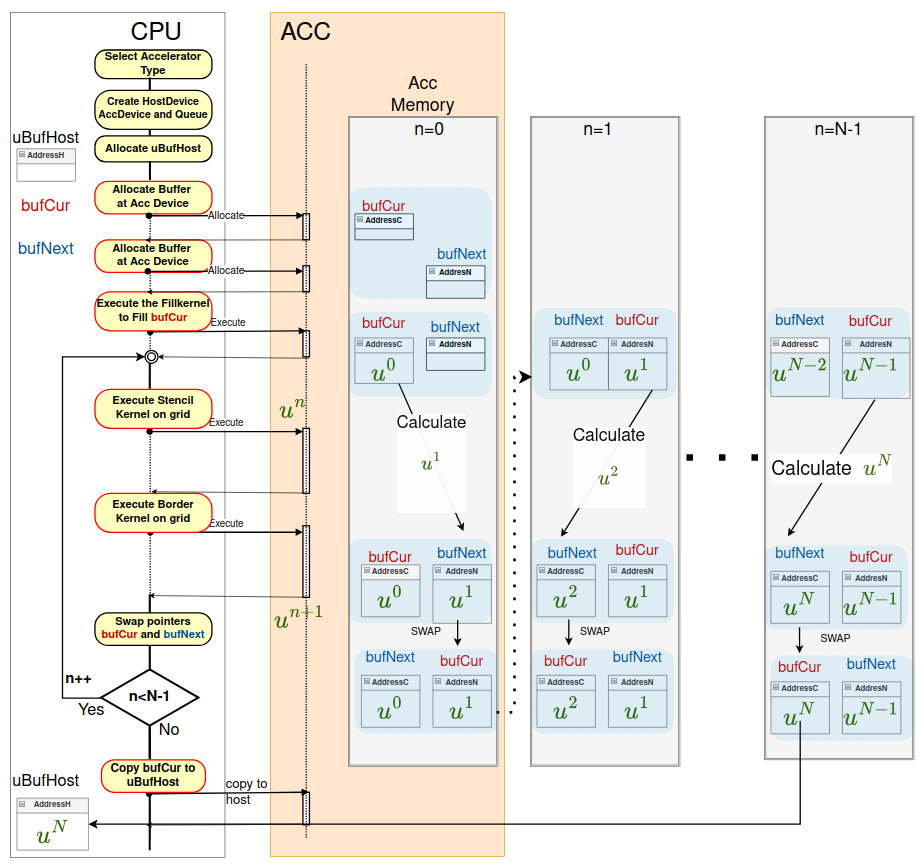
\includegraphics[width=0.92\linewidth,height=0.90\textheight]{Screenshot from 2024-09-26 15-13-53.png}
\end{figure}
\end{frame}

\subsection{Hands on 4: Stencil Kernel}
\begin{frame}[fragile]
\frametitle{Hands On 4: The Stencil Kernel}
\scriptsize
 \textbf{\textit{What kind of parallelization needed} to calculate  $u_{i,j}^{n+1}$ using $u_{i,j}^{n}$ }


    \begin{itemize}
        \item StencilKernel needs a Work-division to work on domain of all nodes (without halo)
        \item Boundary kernel needs a Workdivision which covers nodes + halo region
        \item Boundary kernel will only use threads corresponding to halo region
    \end{itemize}


\textbf{Coding StencilKernel }


    \begin{itemize}
    \item \textbf{Input:} Check the size of the input buffer, it should include halo region as well
    \item \textbf{Thread Index:} Find thread index in the kernel. This index will be used as the center of 3x3 stencil.
    \item \textbf{Memory Adress in Buffer:} Calculate the corresponding memory adress in buffer using thread index. Take into account pitch and data-size
    \item \textbf{Find Stencil matrix} Use dx, dy, dt to calculate the stencil matrix
    \item \textbf{Calculate new heat value:} Calculate $u_{i,j}^{n+1}$ using \textbf{Frobenious Inner Product} of 3x3 matrices
    \item \textbf{Set Value at the Adress:} Set the data at the memory adress.
    \end{itemize}
    \lstset{basicstyle=\ttfamily\tiny}
    \begin{lstlisting}
struct StencilKernel
{
    template<typename TAcc, typename TDim, typename TIdx>
    ALPAKA_FN_ACC auto operator()(
        TAcc const& acc,
        double const* const uCurrBuf, double* const uNextBuf,
        alpaka::Vec<TDim, TIdx> const chunkSize,
        alpaka::Vec<TDim, TIdx> const pitchCurr, alpaka::Vec<TDim, TIdx> const pitchNext,
        double const dx,double const dy, double const dt) const -> void
    {
        ...
    }
};
    \end{lstlisting}
\end{frame}

%\begin{frame}[fragile]
%\frametitle{Applying Boundary Conditions in Parallel}
%\scriptsize
%\textbf{Boundary Kernel:} Ensures correct values at the boundaries of the grid.
%\lstset{basicstyle=\ttfamily\tiny}
%    \begin{lstlisting}
%         // Get indexes
%        auto const gridBlockIdx = alpaka::getIdx<alpaka::Grid, alpaka::Blocks>(acc);
%        auto const blockThreadIdx = alpaka::getIdx<alpaka::Block, alpaka::Threads>(acc);
%        auto const threadIdx1D = alpaka::mapIdx<1>(blockThreadIdx, blockThreadExtent)[0u];
%        auto const blockStartIdx = gridBlockIdx * chunkSize;

%        // Lambda function to apply boundary conditions
%        auto applyBoundary = [&](auto const& globalIdxStart, auto const length, bool isRow)
%        {
%            for(auto i = threadIdx1D; i < length; i += numThreadsPerBlock)
%            {
%                auto idx2D = globalIdxStart + (isRow ? alpaka::Vec<Dim, Idx>{0, i} : alpaka::Vec<Dim, Idx>{i, 0});
%                auto elem = getElementPtr(uBuf, idx2D, pitch);
%                *elem = exactSolution(idx2D[1] * dx, idx2D[0] * dy, step * dt);
%            }
%        };

%        // Apply boundary conditions for the top row
%        if(gridBlockIdx[0] == 0)
%        {
%            applyBoundary(blockStartIdx + alpaka::Vec<Dim, Idx>{0, 1}, chunkSize[1], true);
%        }
%    \end{lstlisting}

%\end{frame}

\begin{frame}
\frametitle{Hands-On Session}
\begin{center}
      \Huge \textbf{Hands-on Session4: Stencil Kernel to Calculate $u^{n+1}$}
  \end{center}
\end{frame}

\section{Setting up the stage to run kernels}
\subsection{alpaka Data Structures}
\begin{frame}
\frametitle{alpaka Data Structures}
\begin{center}
      \Huge \textbf{Setting up the stage to run kernels}
  \end{center}
\begin{enumerate}
 \item Selecting the accelerator and host devices
 \item Allocating and setting host and accelerator device memory
 \item Alpaka Vector, Buffer and View
 \item Passing data to the accelarator
 \item WorkDiv
 \item Define Queue
\end{enumerate}
    \end{frame}


%------------------------------------------------
% mention dont provide code or detailed info
\begin{frame}[fragile]
\frametitle{Accelerator, Device and Host}
\textbf{Define number of dim and index type}
\begin{lstlisting}
using Dim = alpaka::DimInt<2u>; // Number of dim: 2 as a type
using Idx = std::size_t; // Index type of the threads and buffers
\end{lstlisting}

\textbf{Define the accelerator}
\begin{lstlisting}
// AccGpuCudaRt, AccGpuHipRt, AccCpuThreads, AccCpuSerial,
// AccCpuOmp2Threads, AccCpuOmp2Blocks, AccCpuTbbBlocks
using Acc = alpaka::AccGpuHipRt<Dim, Idx>;
using DevAcc = alpaka::Dev<Acc>;
\end{lstlisting}
\textbf{Select a device from platform of Acc}
\begin{lstlisting}
auto const platform = alpaka::Platform<Acc>{};
auto const devAcc = alpaka::getDevByIdx(platform, 0);
\end{lstlisting}
\textbf{Select a host and hostype to allocate memory for data}
\begin{lstlisting}
// Get the host device for allocating memory on the host.
auto const platformHost = alpaka::PlatformCpu{};
auto const devHost = alpaka::getDevByIdx(platformHost, 0);
// Host device type is needed, still not known
using DevHost = alpaka::DevCpu;
\end{lstlisting}
\end{frame}

\begin{frame} [fragile]
\frametitle{What is Accelerator}
\textbf{Accelerator} hides hardware specifics behind alpaka’s abstract API
\lstset{basicstyle=\ttfamily\scriptsize}
\begin{itemize}
\item \textbf{On Host:} Accelerator is a type. A Meta-parameter for choosing correct physical device and dependent types
\begin{lstlisting}
using Acc = acc::AccGpuHipRt<Dim, Idx>;
 \end{lstlisting}
\item \textbf{Inside Kernel:} Accelerator is a variable. Contains thread state, provides access to alpaka’s device-side API
\begin{itemize}
\item The Accelerator provides the means to access to the indices
 \begin{lstlisting}
// get thread index on the grid
auto gridThreadIdx = alpaka::getIdx<Grid, Threads>(acc);
 \end{lstlisting}
\item The Accelerator gives access to alpaka’s shared memory (for threads inside the same block)
 \begin{lstlisting}
// allocate a variable in block shared static memory
auto& sdata = alpaka::declareSharedVar<double[T_SharedMemSize1D], __COUNTER__>(acc);
 \end{lstlisting}
\item Enables synchronization on the block level
 \begin{lstlisting}
// synchronize all threads within the block
alpaka::syncBlockThreads(acc);
 \end{lstlisting}
 \item Maps all device-side functions to their native counterparts
 \begin{lstlisting}
alpaka::sqrt(acc, val); // or atomics, create distribution
 \end{lstlisting}
\end{itemize}
\end{itemize}

\end{frame}

\begin{frame} [fragile]
\frametitle{What is alpaka Buffer, Vector and View}
\begin{itemize}
 \item \textbf{alpaka::Buf} is multi-dimensional dynamic (runtime sized) container.
 \begin{itemize}
 \item Contains \textbf{memory adress, extent, datatype} and the \textbf{device} that memory belongs to!
 \item Device to device copy is easy
 \item Supports [] operator but not [][].
 \lstset{basicstyle=\ttfamily\scriptsize}
 \begin{lstlisting}
 // Allocate buffers
 auto bufCpu = alpaka::allocBuf<float, Idx>(devCpu, extent);
 auto bufGpu = alpaka::allocBuf<float, Idx>(devGpu, extent);
 ....
 // Copy buffer from CPU to GPU. Notice: destination comes first!
 alpaka::memcpy(gpuQueue, bufGpu, bufCpu);
 // cuda way: cudaMemcpy(b_d, b_host, sizeof(float)*N, cudaMemcpyHostToDevice);
 \end{lstlisting}
 \end{itemize}
 \item \textbf{alpaka::Vec} is a static 1D array.
 \begin{lstlisting}
 alpaka::Vec<SizeOfArrayAsType,DataT> myVec;
 \end{lstlisting}
 \item \textbf{alpaka::View} is a non-owning view to an already allocated memory, so that it can be used in alpaka::memcpy
\end{itemize}
    \end{frame}

\subsection{Main accelerator operations}



%------------------------------------------------
% mention dont provide code or detailed info
\subsection{WorkDiv}
\begin{frame}[fragile]
\frametitle{Determining WorkDiv using getValidWorkDiv function}
\textbf{getValidWorkDiv} function calculates blocksize using \textbf{full grid extent!}
\lstset{basicstyle=\ttfamily\scriptsize}
\begin{lstlisting}
    // All kernel inputs are needed because work-division depends on the kernel
    InitializeBufferKernel initBufferKernel;
    // Elements per thread needed to determine work-div
    constexpr alpaka::Vec<Dim, Idx> elemPerThread{1, 1};
    // Give full-grid thread extent as input!
    alpaka::KernelCfg<Acc> const kernelCfg = {extent, elemPerThread};
    // Determine the work-div using kernel and kernel arguments
    auto workDiv = alpaka::getValidWorkDiv(kernelCfg, devAcc, initBufferKernel, uBufAcc.data(), pitchCurrAcc, dx, dy);
\end{lstlisting}
\begin{figure}
    \centering
    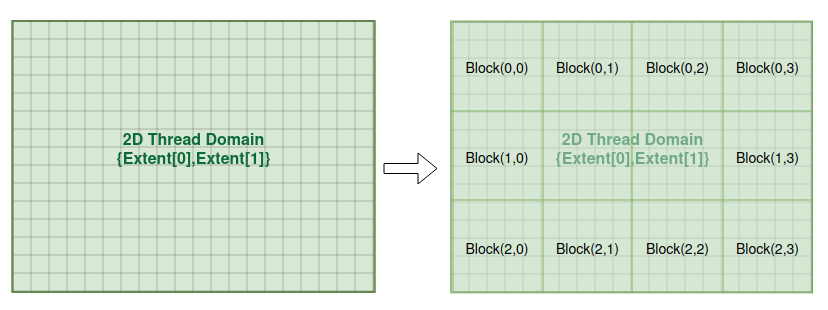
\includegraphics[width=0.75\linewidth]{Screenshot from 2024-10-18 15-16-26.png}
\end{figure}
\end{frame}


\begin{frame}[fragile]
\frametitle{Setting WorkDiv Manually: Set 3 vectors of workdiv}
\begin{lstlisting}
// Set Dim and Index type
using Idx = uint32_t;
using Dim2D = alpaka::DimInt<2u>; // 2 as a type
// 2-element vectors
alpaka::Vec<Dim2D, Idx> gridBlockExtent{M,N}; // 2D grid
alpaka::Vec<Dim2D, Idx> blockThreadExtent{32,32}; // 2D block
alpaka::Vec<Dim2D, Idx> elementExtentPerThread{1,1};
// MxN blocks each has 32x32 threads, each level is 2D
alpaka::WorkDivMembers<Dim2D, Idx> workdiv2D{gridBlockExtent,blockThreadExtent, elementExtentPerThread};
\end{lstlisting}
\begin{figure}
    \centering
    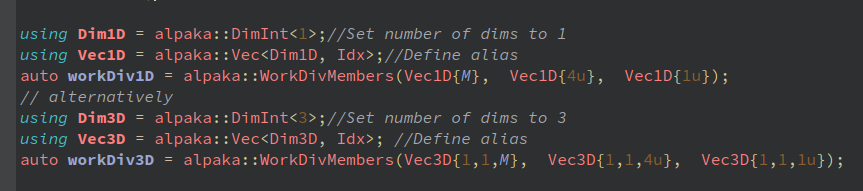
\includegraphics[width=0.75\linewidth]{workdivManual.png}
\end{figure}

\end{frame}



\subsection{Queue}

\begin{frame} [fragile]
\frametitle{What is alpaka::Queue}
\begin{itemize}
 \item \textbf{alpaka::Queue} is “a queue of tasks”.
 \item Used for sycnhronization of tasks like memcpy or kernel-execution
 \item Queue is always FIFO, everything is sequential (in-order) inside the alpaka::queue
 \item If the Queue is \textbf{non-blocking} the caller(host) is not blocked
 \item Different non-blocking queues can run in parallel
 \item Within a single queue accelerator back-ends can be mixed (used in interleaves)
\end{itemize}
\lstset{basicstyle=\ttfamily\scriptsize}
\begin{lstlisting}
// Create queue
using QueueAcc = alpaka::Queue<Acc, alpaka::NonBlocking>;
QueueAcc computeQueue{devAcc};
// Copy host -> device, use the queue
alpaka::memcpy(computeQueue, uCurrBufAcc, uBufHost);
alpaka::wait(computeQueue);  // Not needed, we have single queue
// Create kernel instance
StencilKernel<sharedMemSize> stencilKernel;
// Execute kernel using queue
alpaka::exec<Acc>(computeQueue, workDiv_manual, stencilKernel...)
\end{lstlisting}
\end{frame}

\subsection{Queue Operations}
\begin{frame}[fragile]
\frametitle{Multiple Queues}
\begin{itemize}
\item Queues are used for synchronization

\begin{figure}
    \centering
    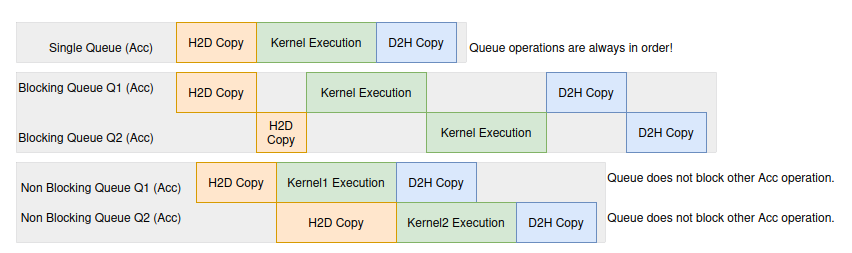
\includegraphics[width=0.8\linewidth]{Screenshot from 2024-10-16 14-52-12.png}
   % \caption{Chunks deviding the domaing and the defined halo regions}
    \label{fig:enter-label}
\end{figure}

\item Copying and processing data synchronously
\begin{lstlisting}
using QueueGpu = alpaka::Queue<AccGpu, alpaka::NonBlocking>;
StencilKernel<sharedMemSize> stencilKernel;
auto queueGpu1 = QueueGpu{devGpu};
auto queueGpu2 = QueueGpu{devGpu};
alpaka::memcpy(queueGpu1, uCurrBufAcc, uBufHost);
alpaka::wait(QueueGpu1);
// Run 2 tasks in parallel: memcpy and exec
alpaka::memcpy(queueGpu2, uCurrBufAcc2, uBufHost2);
alpaka::exec<Acc>(queueGpu1, workDiv_manual, stencilKernel...)
alpaka::wait(QueueGpu1);
alpaka::wait(QueueGpu2);
\end{lstlisting}
\end{itemize}
\end{frame}

\begin{frame}[fragile]
\frametitle{Queue Operations and Tasks}
\begin{itemize}
\item Wrapping an operation as a \textbf{task} is possible.
\begin{lstlisting}
auto const taskRunKernel = alpaka::createTaskKernel<Acc>(workDiv, kernel, /* kernel args */);
auto const taskMemcpy = alpaka::createTaskMemcpy<Acc>( uCurrBufAcc, uBufHost);
\end{lstlisting}
\item Tasks are executed by \textbf{enqueue()} function.
\begin{lstlisting}
alpaka::enqueue(queueA, taskMemCopy);
// taskRunKernel starts after taskMemCopy has finished, even queueA is non-blocking
alpaka::enqueue(queueA, taskRunKernel);
\end{lstlisting}
\item Wait can be used to make queue finish all tasks enqueued
\begin{lstlisting}
// wait until all tasks have completed
alpaka::wait(queueA);
// block queueA until otherQueue has completed
alpaka::wait(queueA, otherQueue);
\end{lstlisting}
\item Queues can be checked for completion of all tasks
\begin{lstlisting}
bool done = alpaka::empty(myQueue);
\end{lstlisting}
\end{itemize}
\end{frame}

\begin{frame}[fragile]
\frametitle{Queue Operations and Events}

\begin{itemize}
%\item
%\item
%\item Tasks on the same queue are executed in order (FIFO principle)
%\begin{lstlisting}
%alpaka::enqueue(queueA, task1);
%alpaka::enqueue(queueA, task2);
%// task2 starts after task1 has finished, even if queueA is non-blocking
%\end{lstlisting}
%\item Order of tasks in different queues is unspecified
%\begin{lstlisting}
%alpaka::enqueue(queueA, task1);
%alpaka::enqueue(queueB, task2);
%// task2 starts before, after or in parallel to task1 if queueA is non blocking
%\end{lstlisting}
\item For easier synchronization, alpaka Events can be inserted before, after or between Tasks:
\begin{lstlisting}
auto myEvent = alpaka::Event<alpaka::Queue>(myDev);
alpaka::enqueue(queueA, myEvent);
alpaka::wait(queueB, myEvent);
// queueB will only resume after queueA reached myEvent
\end{lstlisting}
\end{itemize}
\end{frame}


\begin{frame}
\frametitle{Some sychronization scenarios}
\begin{figure}
    \centering
    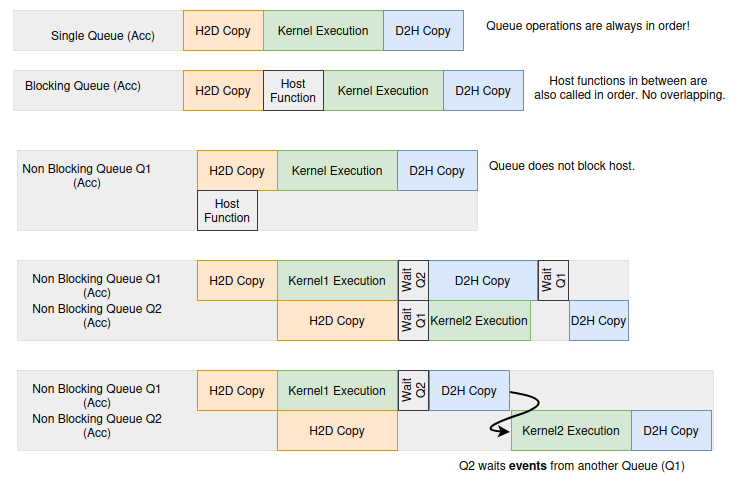
\includegraphics[width=0.93\linewidth]{Screenshot from 2024-10-16 16-53-06.png}
    \label{fig:enter-label}
\end{figure}
\end{frame}



\begin{frame}[fragile]
\frametitle{Going over Kernel execution and copying data}
\begin{itemize}

\item Create the queue and buffer using device
\lstset{basicstyle=\ttfamily\scriptsize}
\begin{lstlisting}
// Create queue,
// queue is needed for kernel execution and copies to/from accelerator
    alpaka::Queue<Acc, alpaka::NonBlocking> queue{devAcc};
    auto uBufAcc = alpaka::allocBuf<float, Idx>(devAcc, extent);
\end{lstlisting}

\item Execute the kernel using the queue, the workdiv and kernel arguments:
\lstset{basicstyle=\ttfamily\scriptsize}
\begin{lstlisting}
    alpaka::exec<Acc>(queue, workDiv, initBufferKernel, uBufAcc.data(), pitchCurrAcc, dx, dy);
\end{lstlisting}
\item Copy the filled buffer back to the host
\begin{lstlisting}
     // Copy device -> host
     // Since buffers know their corresponding devices (host or acc) memcopy does not need any device variable
    alpaka::memcpy(queue, uBufHost, uBufAcc);
    alpaka::wait(queue);
\end{lstlisting}
\end{itemize}
\end{frame}

\section{Optimization of Solution}

\begin{frame}
\frametitle{Optimization and usability}
\begin{center}
      \Huge \textbf{alpaka Usability and Optimization Features}
  \end{center}
\begin{enumerate}
 \item Use alpaka \textbf{mdspan} to set, get, pass data easily (Hands-On 5)
 \item Use \textbf{Domain Decomposition}: Divide the domain into \textbf{chunks} (Hands-On 6)
 \item Use \textbf{2 asynch queues} for performance increase (Hands-On 7)
 \item Use \textbf{shared memory} for performance increase (Hands-On 8)
 %\item Use \textbf{alpaka::UniformElements} for easier indexing
\end{enumerate}
    \end{frame}

\subsection{Hands on 5: MdSpan}
\begin{frame}[fragile]
\small
\frametitle{alpaka::experimental::mdspan}
\textbf{Mdspan a multi-dimensional and non-owning view}
\begin{itemize}
\item Part of C++23 standard. Can be used with C++17.
\item Consists pointer, pitch and data size
\item Has member functions to get/set data and to get extents
 \end{itemize}
 \textbf{Mdspan Installation}
 \begin{itemize}
\item Set $alpaka\_USE\_MDSPAN$ cmake variable to $FETCH$ while installing alpaka
\item Alternatively, set $alpaka\_USE\_MDSPAN$ cmake variable to $FETCH$ while configuring example if it is not already set while installation
\begin{lstlisting}
// in build directory
cmake -Dalpaka_USE_MDSPAN=FETCH ..
 \end{lstlisting}
\end{itemize}
\textbf{Passing mdspan to kernel}
\lstset{basicstyle=\ttfamily\scriptsize}
\begin{lstlisting}
 // Host code: Allocate device memory
 auto bufDevA = alpaka::allocBuf<DataType, Idx>(devAcc, extentA);
 // Create mdspan views for device buffers using alpaka::experimental::getMdSpan
 auto mdDevA = alpaka::experimental::getMdSpan(bufDevA);
 // Execute the kernel
 alpaka::exec<Acc>(queue, workDiv, kernel, mdDevA, mdDevB, mdDevC);
 \end{lstlisting}
 \end{frame}
%------------------------------------------------
\begin{frame} [fragile]
\frametitle{Kernel using mdspan instead of data pointer and pitch}
\lstset{basicstyle=\ttfamily\tiny}

\textbf{Accessing data at host or at accelerator}
 \lstset{basicstyle=\ttfamily\scriptsize}
 \begin{lstlisting}
 struct MatrixAddKernel
 {   template<typename TAcc, typename TMdSpan>
     ALPAKA_FN_ACC void operator()(TAcc const& acc, TMdSpan A, TMdSpan B, TMdSpan C) const
     {
         auto const i = alpaka::getIdx<alpaka::Grid, alpaka::Threads>(acc)[0];
         auto const j = alpaka::getIdx<alpaka::Grid, alpaka::Threads>(acc)[1];
         if(i < C.extent(0) && j < C.extent(1))
         {
                  C(i, j) = A(i, j) + B(i, j);
         }
     } };
 \end{lstlisting}
\begin{lstlisting}
// Update the kernel: Use mdspan instead of pointer+pitch
struct StencilKernel
{
    template<typename TAcc, typename TDim, typename TIdx>
    ALPAKA_FN_ACC auto operator()(
        TAcc const& acc,
        double const* const uCurrBuf, double* const uNextBuf,
        alpaka::Vec<TDim, TIdx> const& pitchCurr,
        alpaka::Vec<TDim, TIdx> const& pitchNext,
        alpaka::Vec<TDim, TIdx> const& haloSize,
        double const dx, double const dy, double const dt) const -> void
        {  .....
        }};

\end{lstlisting}
\end{frame}

\begin{frame}
\frametitle{Hands-On Session}
\begin{center}
      \Huge \textbf{Hands-on Session5: Use mdspan to pass data to kernel}
  \end{center}
\end{frame}
%------------------------------------------------
% Will go down because this is optimization: opt is shared memory, 2 queues
%
\subsection{Hands on 6: Domain Decomposition}
\begin{frame}
\frametitle{Chunk Definition}
\textbf{Chunk:} Subdomains needed for latency management of block level parallelisation
\vspace{-0.5\baselineskip}
\begin{figure}
    \centering
    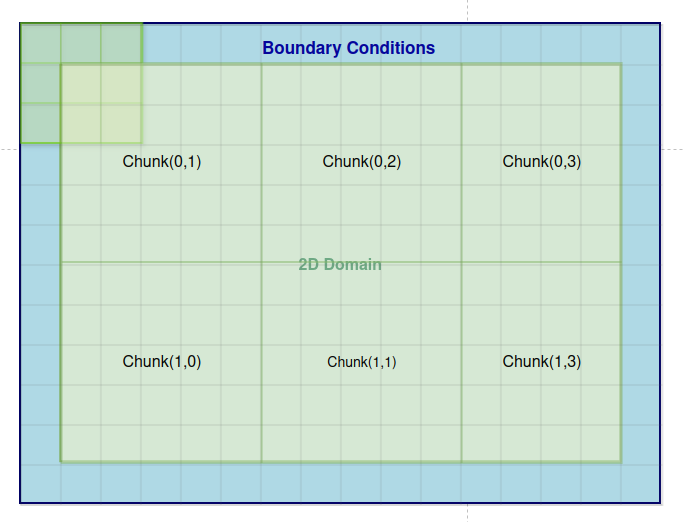
\includegraphics[height=0.78\textheight]{Screenshot from 2024-09-02 14-11-22.png}
    \label{fig:enter-label}
\end{figure}
\end{frame}

\begin{frame}
\frametitle{Calculation by a block of grids of stencil kernel}
\begin{itemize}
%    \item \textbf{Halo Region For Shared:} A layer of block cells surrounding the main computational domain.

    \item Chunking is a Domain Decomposition method
    \item A block of threads update a chunk of heat data
    \item A grid of threads updates the whole domain
\end{itemize}
\begin{figure}
    \centering
    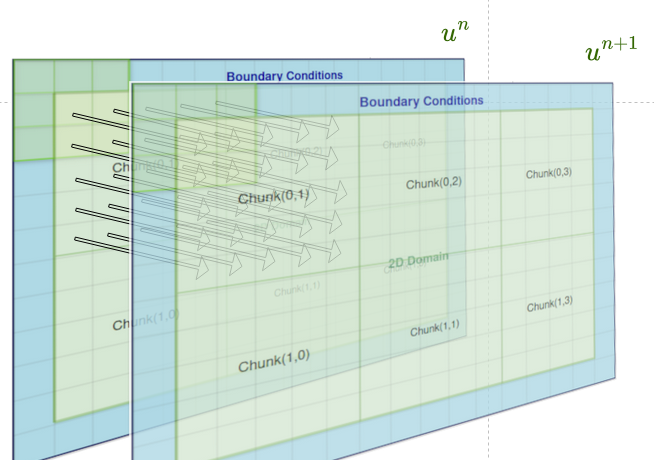
\includegraphics[width=0.75\linewidth]{Screenshot from 2024-09-04 13-55-10.png}
\end{figure}
\end{frame}

\begin{frame}
\frametitle{Chunks in Parallel Grid Computations}
\begin{itemize}
%    \item \textbf{Halo Region For Shared:} A layer of block cells surrounding the main computational domain.
    \item \textbf{Halo Region around chunk:} A layer of grid cells surrounding the subdomains.
    \item \textbf{Halo Size:} Typically 1 for a 5-point stencil.
    \item Chunks-size could be larger than the block size.
\end{itemize}

\begin{figure}
    \centering
    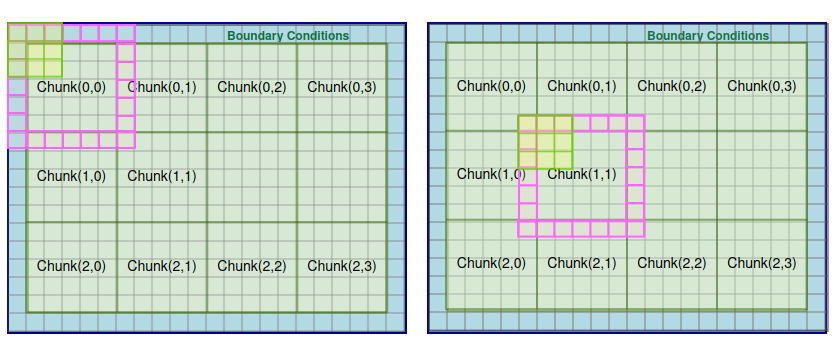
\includegraphics[width=0.8\linewidth]{Screenshot from 2024-08-30 19-03-50.png}
   % \caption{Chunks deviding the domaing and the defined halo regions}
    \label{fig:enter-label}
\end{figure}
\end{frame}




\begin{frame}
\frametitle{A block is responsible from a chunk}
\begin{figure}
    \centering
    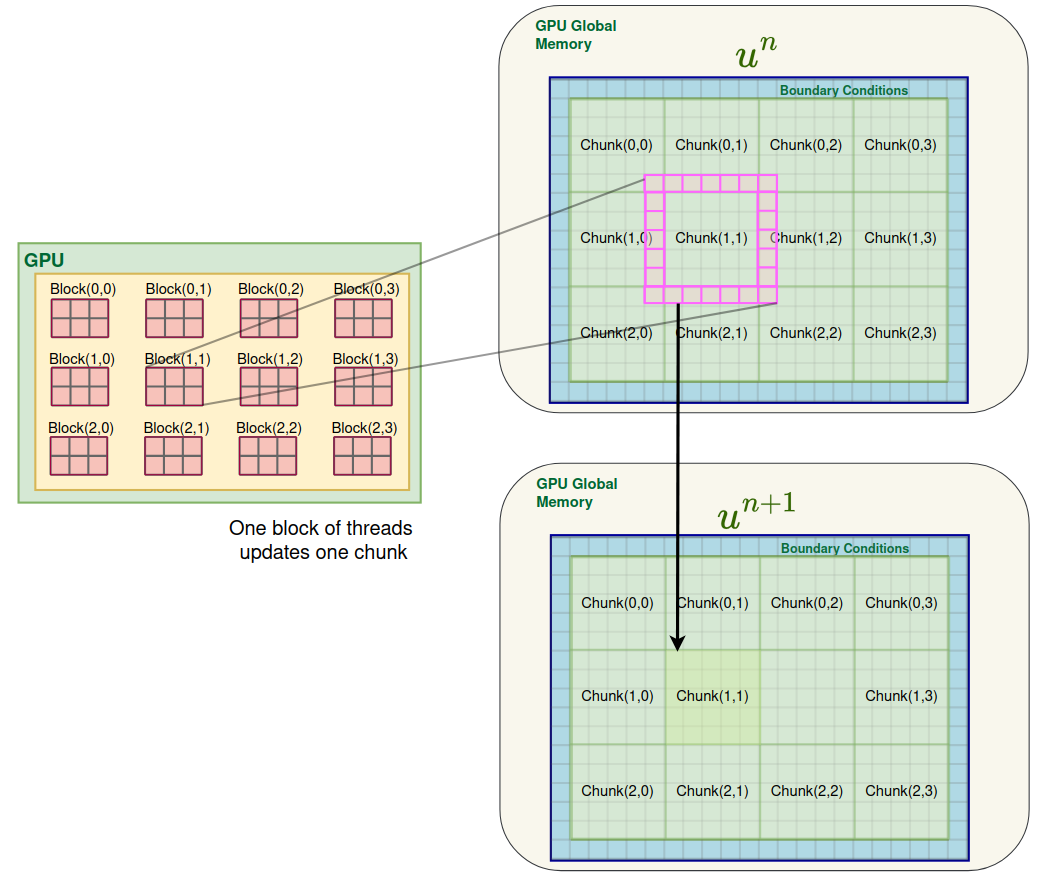
\includegraphics[height=0.9\textheight]{Screenshot from 2024-10-01 12-51-51.png}
   % \caption{Chunks deviding the domaing and the defined halo regions}
    \label{fig:enter-label}
\end{figure}
\end{frame}

\begin{frame}[fragile]
\frametitle{Determine WorkDiv for Chunked Solution}

\textbf{Set work division fields directly:}
\lstset{basicstyle=\ttfamily\scriptsize}
\begin{lstlisting}
// Define a workdiv for the shared memory based heat eqn solution
constexpr alpaka::Vec<Dim, Idx> elemPerThread{1, 1};
// Get max threads that can be run in a block for this kernel
auto const kernelFunctionAttributes = alpaka::getFunctionAttributes<Acc>(
    devAcc,
    stencilKernel,
    uCurrBufAcc.data(), uNextBufAcc.data(),
    chunkSize,
    pitchCurrAcc,pitchNextAcc,
    dx,dy, dt);
auto const maxThreadsPerBlock = kernelFunctionAttributes.maxThreadsPerBlock;
auto const threadsPerBlock
    = maxThreadsPerBlock < chunkSize.prod() ? alpaka::Vec<Dim, Idx>{maxThreadsPerBlock, 1} : chunkSize;
alpaka::WorkDivMembers<Dim, Idx> workDiv_manual{numChunks, threadsPerBlock, elemPerThread};
\end{lstlisting}
\end{frame}

\begin{frame}
\frametitle{Hands-On Session}
\begin{center}
      \Huge \textbf{Hands-on Session6: Optimized Heat Eqn. solution by Domain Decomposition}
  \end{center}
\end{frame}

%------------------------------------------------
\subsection{Hands on 7: Parallel Queues}
\begin{frame}
\frametitle{Running 2 parallel queues: Additional queue to dump temporary results}
\begin{columns}
  \begin{column}{0.63\textwidth}
\begin{itemize}
 \item Create an additional alpaka::queue instance at accelerator to run parallely
 \item The temporary heat result $u^{n}$ will be copied to host from accelerator at the end of each iteration
 \item Copying can start while the stencil and boundary kernels are running
 \item In order to run 2 queues paralelly they should be a NonBlocking queues
 \item The copied heat data will be used to create an animation of images
\end{itemize}
  \end{column}

  \begin{column}{0.37\textwidth}
\begin{figure}
    \centering
    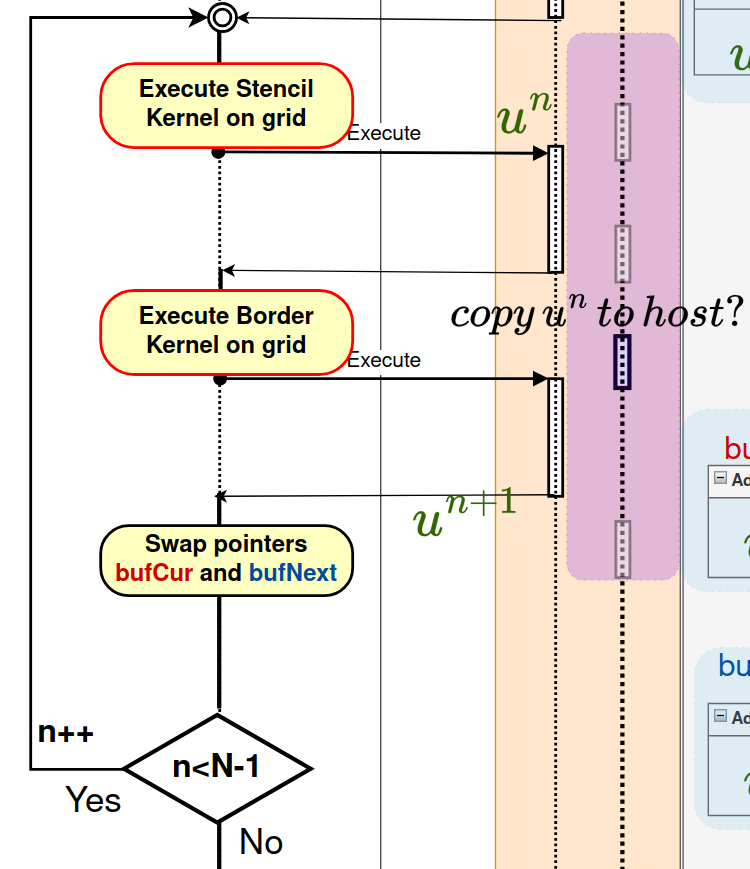
\includegraphics[width=0.99\linewidth]{Screenshot from 2024-09-26 15-53-41.png}
   % \caption{Chunks deviding the domaing and the defined halo regions}
   % \label{fig:enter-label}
\end{figure}
  \end{column}
  \end{columns}
\end{frame}

\begin{frame}
\frametitle{Current Loop}
\begin{figure}
    \centering
    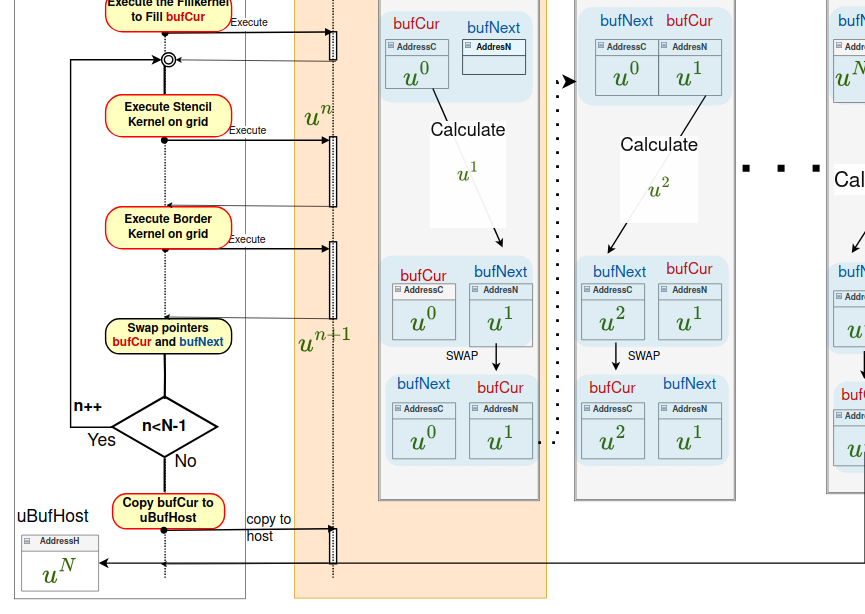
\includegraphics[width=0.8\linewidth]{Screenshot from 2024-09-26 14-33-46.png}
   % \caption{Chunks deviding the domaing and the defined halo regions}
   % \label{fig:enter-label}
\end{figure}
\end{frame}

\begin{frame}
\frametitle{Copy $u^{n}$ back at each iteration sequentially}
\begin{figure}
    \centering
    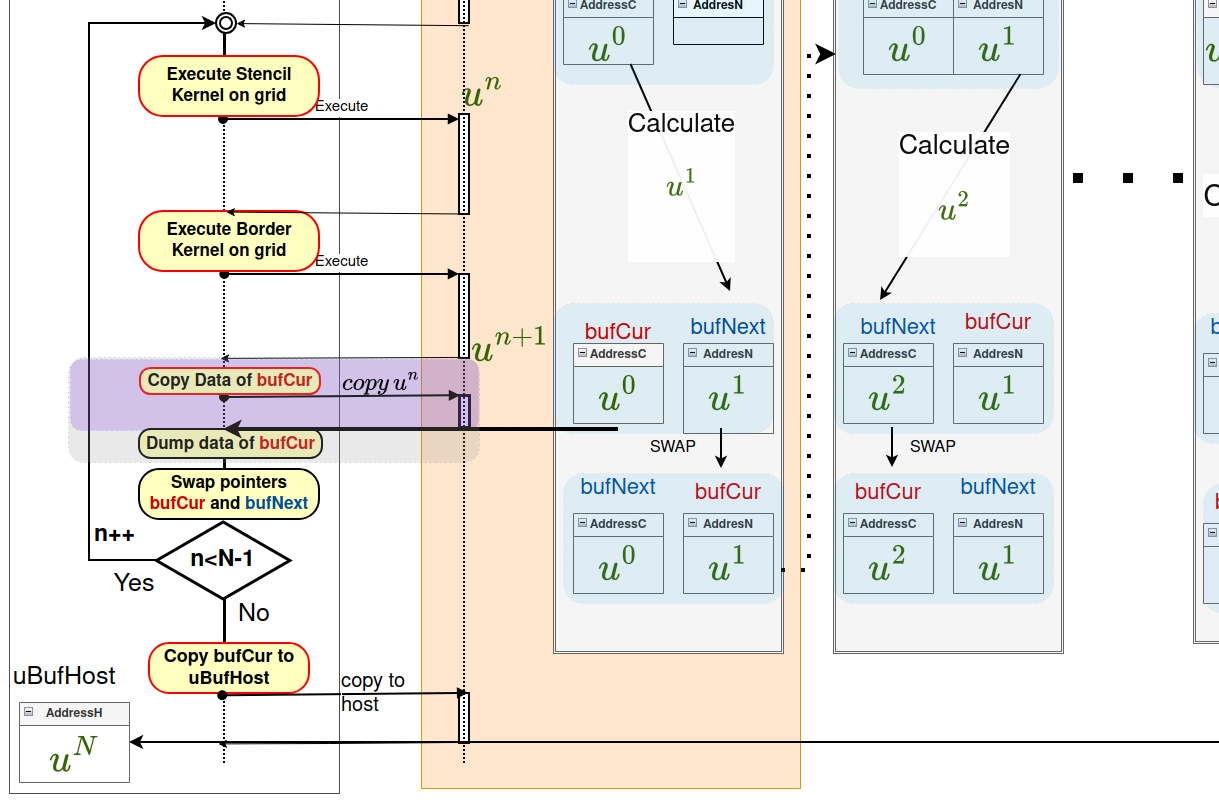
\includegraphics[width=0.8\linewidth]{Screenshot from 2024-09-26 15-05-08.png}
   % \caption{Chunks deviding the domaing and the defined halo regions}
    \label{fig:enter-label}
\end{figure}
\end{frame}

\begin{frame}
\frametitle{Hands on 7: Copy $u^{n}$ back at each iteration while kernel is running}
\begin{figure}
    \centering
    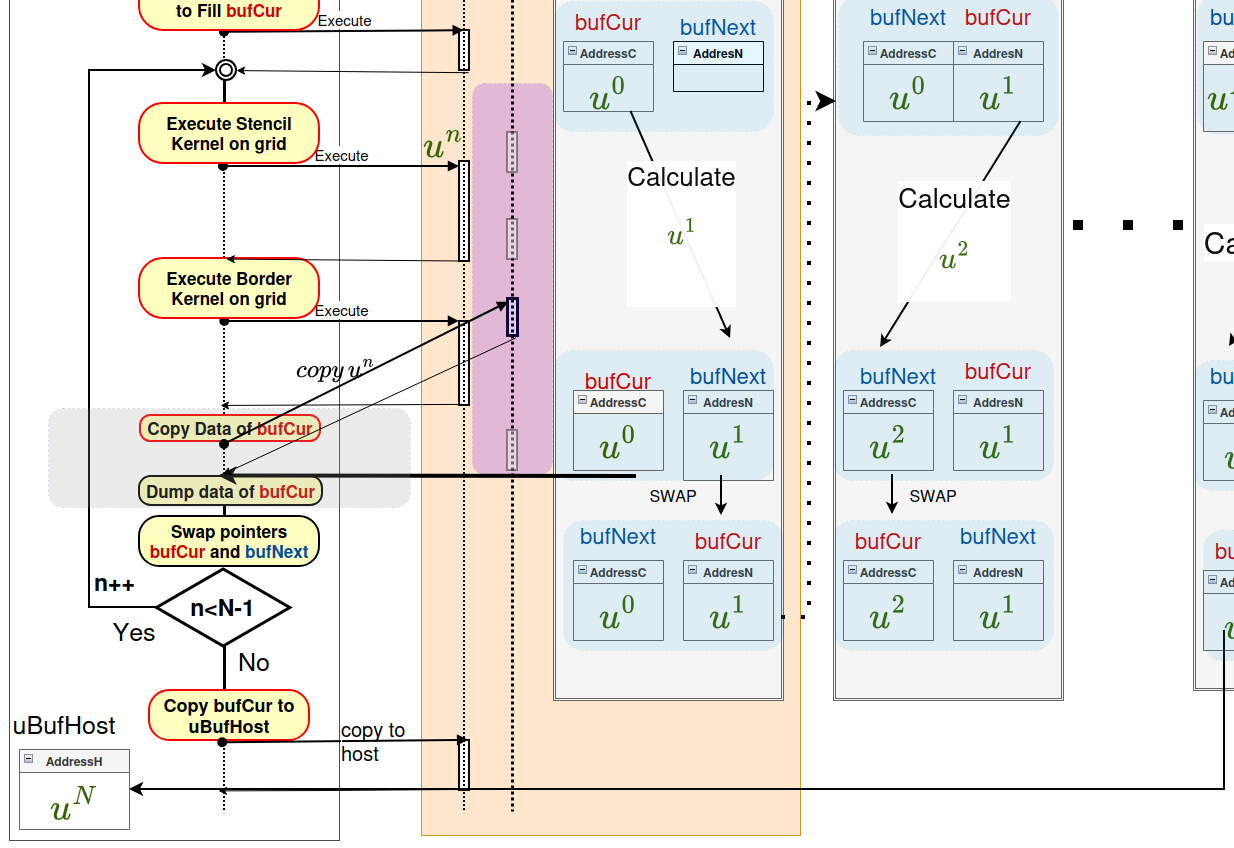
\includegraphics[width=0.8\linewidth]{Screenshot from 2024-10-17 16-11-14.png}
   % \caption{Chunks deviding the domaing and the defined halo regions}
    \label{fig:enter-label}
\end{figure}
\end{frame}

%------------------------------------------------

\begin{frame}
\frametitle{Hands-On Session}
\begin{center}
      \Huge \textbf{Hands-On Session7: Running 2 parallel queues to dump heat at each step}
  \end{center}
\end{frame}
\subsection{Hands on 8: Shared Memory}

%% Cizim yap gercek sizelar olabilir
\begin{frame}[fragile]
\frametitle{Efficient Stencil Application with Shared Memory}
\begin{columns} %[T] % The [T] option aligns the tops of the columns
\vspace{-1.3cm}
\hspace*{-0.6cm} % Adjust the -1cm to move more or less to the left
% First Column
\begin{column}{0.56\textwidth}

\textbf{Shared Memory at GPUs}
    \begin{itemize}
        \item A fast, limited-size memory accessible by all threads within a block.
        \item Faster than global memory. Stores data at CU (or SM).
        \item Shared Memory allocation can be static or dynamic.
         \item Filling shared memory is done by the same kernel calculating the stencil
         \item Threads in a block must synchronize to ensure all data is loaded into shared memory before computation begins.
   \end{itemize}
\end{column}
\begin{column}{0.44\textwidth}
\begin{figure}
    \centering
    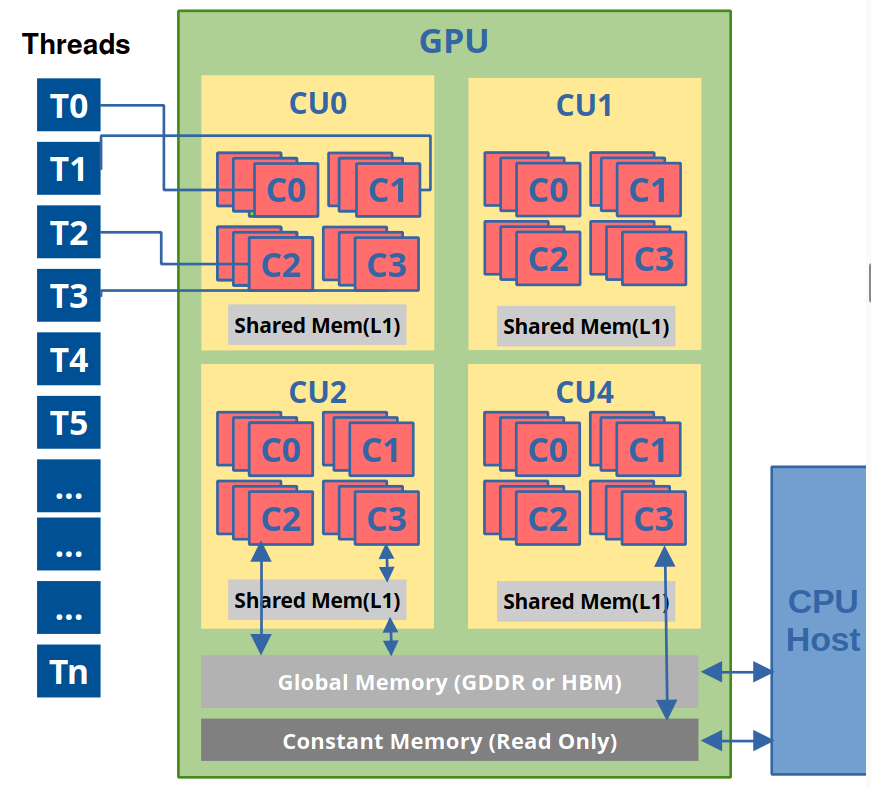
\includegraphics[width=0.96\linewidth]{Screenshot from 2024-10-18 20-08-56.png}
   % \caption{Chunks deviding the domaing and the defined halo regions}
    \label{fig:enter-label}
\end{figure}

\end{column}
\end{columns}

\end{frame}


\begin{frame}
\frametitle{Shared memory data: chunk with halo}
\begin{itemize}
%    \item \textbf{Halo Region For Shared:} A layer of block cells surrounding the main computational domain.
    \item \textbf{Halo Region around chunk:} A layer of grid cells surrounding the subdomains. In order to use the heat value beside the current chunk
    \item \textbf{Halo Size:} Typically 1 for a 5-point stencil.
    \item Chunks might include more than one blocks depending on the blocksize
    \item Kernel will install the data to shared memory then use the data from shared memory
\end{itemize}

\begin{figure}
    \centering
    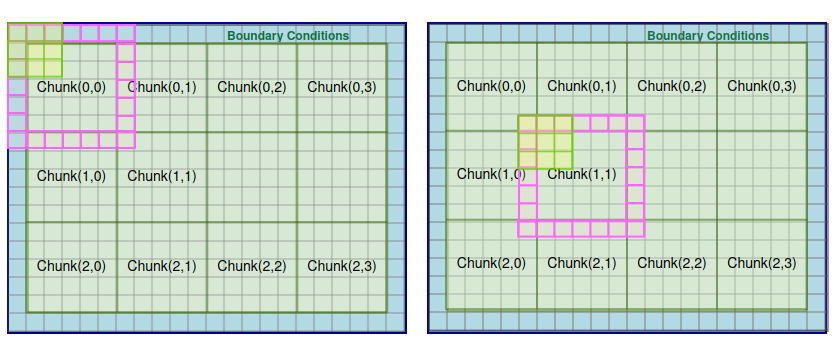
\includegraphics[width=0.8\linewidth]{Screenshot from 2024-08-30 19-03-50.png}
   % \caption{Chunks deviding the domaing and the defined halo regions}
    \label{fig:enter-label}
\end{figure}
\end{frame}

\begin{frame}
\frametitle{Finding $u^{n+1}$ by using $u^{n}$ from chunks at shared memory}
\begin{figure}
    \centering
    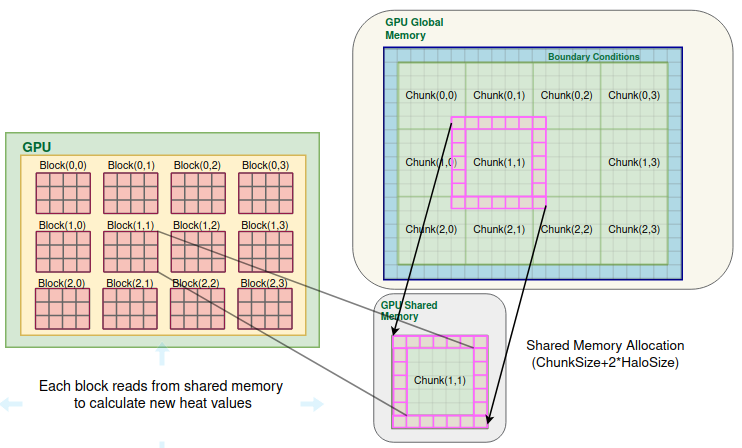
\includegraphics[width=0.9\linewidth]{Screenshot from 2024-10-01 13-19-49.png}
   % \caption{Chunks deviding the domaing and the defined halo regions}
    \label{fig:enter-label}
\end{figure}
\end{frame}

\begin{frame}
\frametitle{Kernel Operations of a Block to Find $u^{n+1}$ for block data}
\begin{figure}
    \centering
    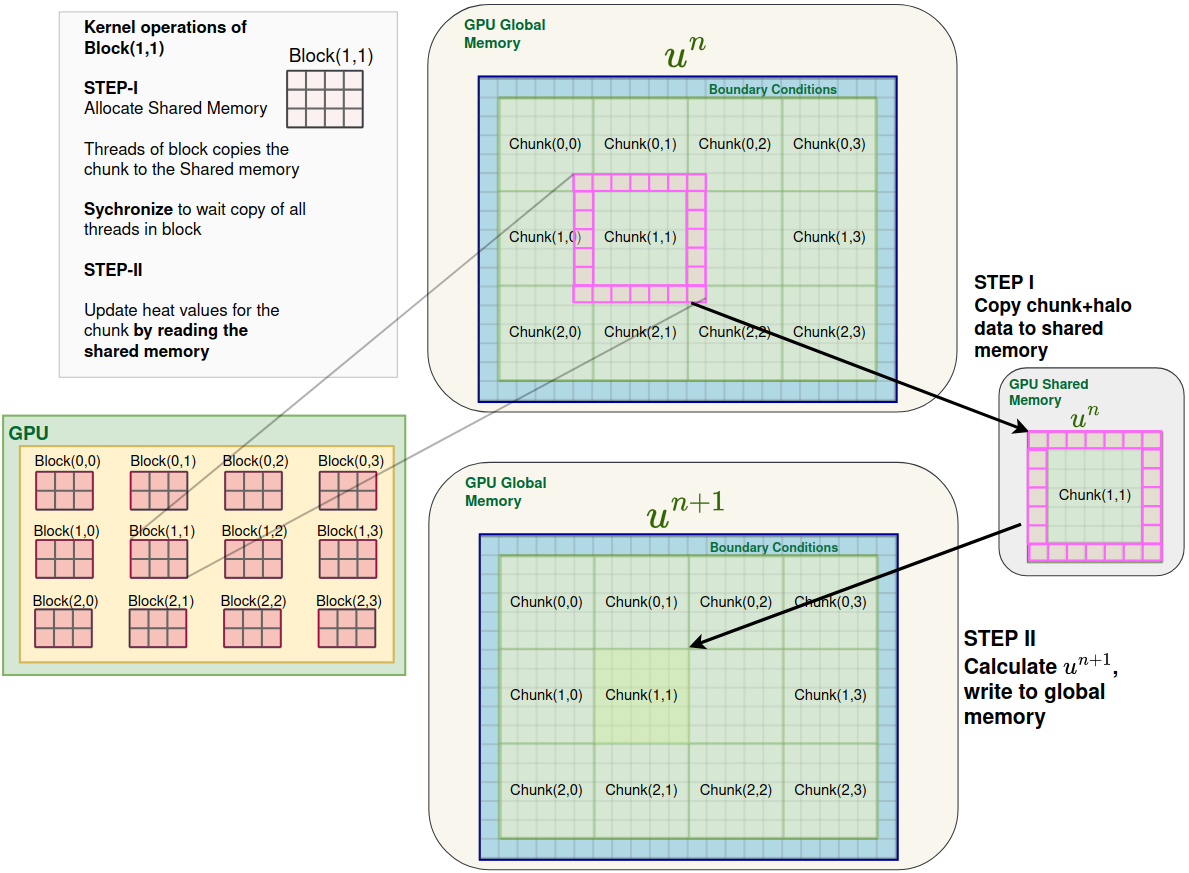
\includegraphics[width=0.9\linewidth]{Screenshot from 2024-10-01 12-57-11.png}
   % \caption{Chunks deviding the domaing and the defined halo regions}
    \label{fig:enter-label}
\end{figure}
\end{frame}

\begin{frame}[fragile]
\frametitle{Hands on 8: Stencil Kernel using shared memory}
\begin{itemize}
    \item \textbf{Allocate shared memory inside kernel}
   \lstset{basicstyle=\ttfamily\scriptsize}
     \begin{lstlisting}
     // Allocate shared memory inside kernel, this will be done only once per block although it is in the kernel
     // Size is determined in compile time and is passed to kernel as a type
      auto& sdata = alpaka::declareSharedVar<double[T_SharedMemSize1D], __COUNTER__>(acc);
        \end{lstlisting}
 \item \textbf{Calculate thread index}
  \item \textbf{Fill the shared memory by block of threads}
 \item \textbf{Wait for shared memory to be filled by all block threads}
 \begin{lstlisting}
       alpaka::syncBlockThreads(acc);
   \end{lstlisting}
 \item \textbf{Calculate new heat value using the data from the shared memory}
 \item \textbf{Set the new heat value}
 \end{itemize}
\end{frame}







\begin{frame}
\frametitle{Hands-On Session}
\begin{center}
      \Huge \textbf{Hands-on Session8: Optimized Heat Eqn. solution by using shared memory}
  \end{center}
\end{frame}


%------------------------------------------------
%------------------------------------------------
\section{Conclusion}
%------------------------------------------------
\subsection{Summary}
\begin{frame}
\frametitle{Conclusion: Parallel Techniques For Solving Heat Equation}
\begin{itemize}
    \item \textbf{Kernel Definition}
    \begin{itemize}
        \item Kernel to fill a buffer in parallel
        \item Stencil Kernel for calculating the next set of heat values
        \item Boundary Kernel
    \end{itemize}
    \item \textbf{Work division}
    \begin{itemize}
        \item Getting a valid work division according to accelerator
        \item Setting work-division manually
    \end{itemize}
    \item \textbf{Allocating and Setting Memory at Host and Accelerator }
    \begin{itemize}
        \item Using alpaka::buffer
        \item Using alpaka::memcpy
    \end{itemize}
    \item \textbf{Alpaka Structures}
    \begin{itemize}
        \item Accelerator, Device, Queue, Task
    \end{itemize}
    \item \textbf{Optimizations and Usability}
    \begin{itemize}
        \item Using alpaka Mdspan
        \item Domain Decomposition
        \item Using Multiple Async Queues
        \item Using GPU's Shared Memory
    \end{itemize}
\end{itemize}
\end{frame}

%------------------------------------------------
\subsection{Questions}
\begin{frame}
\Huge{\centerline{End of Alpaka Hackathon.}}
\Huge{\centerline{Any Questions?}}
\end{frame}

%----------------------------------------------------------------------------------------

\end{document}
